\section{Evaluation}

To evaluate a system, it is necessary to have access to metrics to quantify its performance.In the case of machine learning algorithms, the most important metric is Error.

\subsection{True vs Empirical Error}
The error that we can observe, the \textbf{Empirical Error}, is the one related to the training set available to us, and it can vary from set to set. The \textbf{Actual Error}, on the other hand, is generally unknown to us and is the classification error of all possible examples.

\subsubsection{Example}
\begin{itemize}
    \item[\textcolor{green!50!black}{\textbullet}] Correctly classified: $f(x) = h(x)$
    \item[\textcolor{red}{\textbullet}] Misclassified: $f(x) \not= h(x)$
\end{itemize}
\begin{center}
    \begin{tabular}{c}
        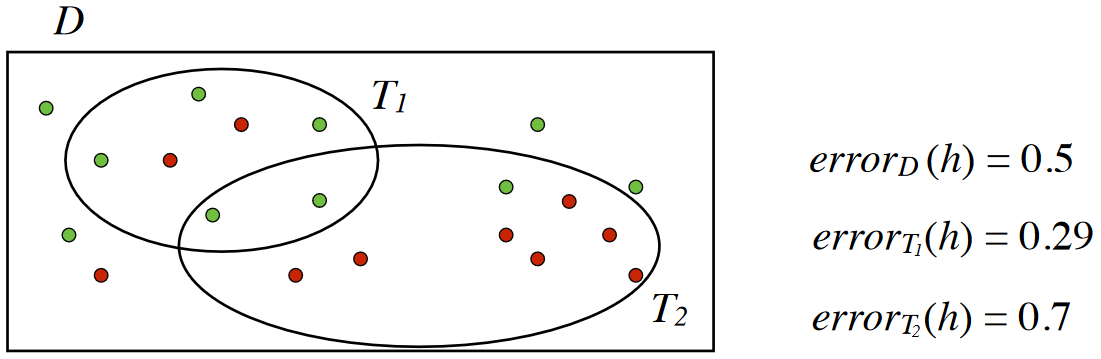
\includegraphics[width=0.8\textwidth]{images/Error.png}
    \end{tabular}
\end{center}
Depending on the training set the model may have too much bias or have too much variance.  In the image the $T_1$ set of examples leads the model to have too much optimistic bias, the $T_2$ set on the contrary has too much variance and therefore any corrections are likely to be detrimental to the model because they will increase the bias or variance in the wrong directions.  To improve our assessment of model performance it is important to make sure that the \textbf{Empirical Error} is as close as possible to the \textbf{True Error}.

\subsection{Model Selection}

\subsubsection{Hold-out}

\subsubsection{K-fold Cross Validation}

\subsubsection{Leave-one-out}


\newpage